\chapter{Machine Learning and \mbox{uncertainties}}
\label{methods_ML}

\vspace{-15pt} % one line spacing corresponds approx to 15 pts
\begin{tcolorbox}[enhanced,width=\textwidth,size=fbox,
        sharp corners,colframe=black!5!white,drop fuzzy shadow southeast,
        boxrule=3mm, parbox=false] 
        
This chapter borrows from the article \citep{walch_big_2020}:

\qquad \bibentry{walch_big_2020}

and the conference proceedings \cite{walch_spatio-temporal_2019, walch_fast_2019}:

\quad \bibentry{walch_spatio-temporal_2019} 

\quad \bibentry{walch_fast_2019}
\end{tcolorbox}

The large-scale estimation of HyREP at high spatial and temporal resolution challenges the analytical and geospatial models from Chapter~\ref{methods_physical}, for three main reasons.
First, some data required to perform the analytical and geospatial modelling may not be available across the entire region for which the HyREP is computed.
Second, the resolution or quality of some of the input datasets may be insufficient to assure a high-resolution potential estimation, but it could be improved through the use of additional information.
Third, these physics-based approaches may be too computationally intensive, inhibiting their application at the large scale.
The use of Machine Learning (ML) as a method to address the above limitations of "classical" physics-based models has attracted increasing attention in recent years \cite{willard_integrating_2020}. 

In this thesis, we use ML to address several of the above-mentioned limitations for the national-scale estimation of RPV (Chapter~\ref{solar}) and GSHP (Chaper~\ref{geothermal}) potential. 
The ML models hereby % To this aim, ML is used in two contexts: 
% (i) To 
learn and predict the relationship between a set of input data (\textit{features}) and output variables (\textit{targets}), known as \textit{supervised learning}, 
% and (ii) to group data based on similarities in its features and to identify outliers, known as \textit{clustering}. 
as summarized in Section~\ref{ML_supervised}.
For an in-depth introduction to Machine Learning, interested readers may refer for example to \citet{bishop_pattern_2006}.
\nomenclature[A]{ML}{Machine Learning}

The use of data-driven methods further requires the estimation of \textit{uncertainties} related to the ML predictions, which are essential for decision-making processes \cite{knusel_argument-based_2020}. 
Uncertainties may arise for example from noise in input data sources or from the modelling approaches themselves, and their quantification is a vast field of research \cite{willard_integrating_2020,knusel_argument-based_2020}.
We model uncertainties arising from data noise and from ML models in the form of standard deviations, which we propagate through the analytical models presented in Chapter~\ref{methods_physical}. 
% The following sections will provide an overview of the supervised learning  and clustering techniques used in this thesis, as well as 
Section~\ref{unc} provides an overview of the applied methods for a systematic quantification of uncertainties through combined physics-based and data-driven modelling approaches. 

\section{Supervised learning}
\label{ML_supervised}

Supervised learning algorithms are trained on a set of input features and corresponding output targets, such as to minimise the error between an algorithm's prediction and the "true" target.
Several design choices can influence the performance of supervised learning algorithms: (i) the choice of the input features, (ii) the choice of an appropriate ML model for a given problem, and (iii) the
choice of the parameters defining the model structure (hyper-parameters).
The selection of suitable input features varies largely between different ML applications and is often based on expert knowledge. 
The full set of available features, obtained using expert knowledge or otherwise, may however contain features which are redundant or even detrimental to the ML model's performance.
Feature exploration and selection techniques may hence be used to enhance the quality of the feature set (Section~\ref{ML_features}).

The choice of an appropriate ML model depends on the structure of the problem and the available data. Regression algorithms are used to model continuous targets, while classification algorithms are used for binary or multi-class targets (see Section~\ref{ML_models}). Furthermore, some algorithms such as Support Vector Machines (SVM) may be better suited for high-dimensional feature sets (i.e. many features), while other algorithms such as Extreme Learning Machines (ELM) are optimized for very large datasets. For image or natural language processing, convolutional neural networks (CNNs) have gained high popularity in recent years.
% For many applications, however, multiple algorithms may be appropriate and their performance should be compared to choose the best model.

For any ML model, the optimization of its hyper-parameters is performed during the so-called \textit{tuning} procedure in the training phase. For model training, the labelled data (all data samples for which both features and targets are known) are divided into three random subsets: 
(i) The \textit{training} set, which is used to fit the model, (ii) the \textit{validation} set, which is used to assess the performance during model tuning, and (iii) the \textit{test} set, which is excluded from the tuning procedure and used for the final model evaluation.
The test set usually contains $20 - 33\%$ of the labelled data. The remaining data is then split again, keeping another $20 - 33\%$ for model validation.
To reduce the randomness in the splitting of the data into training and validation sets, a $k$-fold cross-validation (CV) procedure is widely applied in the literature. 
For this, the training data is randomly split into $k$ subsets (folds), from which $k$ ML models are trained. Each model uses ($k$ – 1) folds for training and the last fold for validation. 
Unless mentioned otherwise, we use a 5-fold cross-validation ($k$ = 5) throughout this work.
% 
% Often regarded as black-box models, ML algorithms are trained based on a set of input data (called features), such as to predi ct an output (the target or label). 
% The architecture of each model is determined through a tuning procedure in the training phase, where the parameters defining the model structure (hyper-parameters) are optimized in order to minimize the difference between the prediction and the target. 

\subsection{Feature exploration and selection techniques}
\label{ML_features}

A vast variety of methods exist in the literature for the exploration, analysis and selection of appropriate features for ML models, which are often highly dependent on the application. In this section we introduce five concepts for designing ML feature sets which have proven useful for the ML applications presented in this thesis.

\textbf{Correlation analysis} provides insights into potential redundancies between different features, and allows to obtain a first quantitative measure of the relevance of each feature towards predicting the target variable(s).
In addition to the widely used Pearson correlation coefficient, which measures linear correlations, other measures of non-linear dependencies between variables may be used, such as Spearman's rank correlation coefficient \cite{kokoska_crc_1999} or mutual information \cite{kozachenko_statistical_1987}. While low correlations are desirable between the different features, indicating low redundancy within the feature set, high correlations between the features and the target suggest a high importance towards predicting this target.

\textbf{Feature transformation} includes the normalisation of the features, typically to zero mean and unit variance, but it may further refer to non-linear transformations of the features or the target. While normalisation is standard practice and required for many ML algorithms, the suitability of non-linear transformations depends on the data. For example, log-transformations may significantly improve the predictions for features at exponential scale. Feature visualisation through histograms or scatterplots can provide insights into suitable transformations.

\textbf{Principal Component Analysis (PCA)} \cite{tipping_probabilistic_1999} is an advanced feature transformation technique which yields a set of independent (principal) components. These components are ranked according to the percentage of explained variance in each component. To select features using PCA, the minimum percentage of explained variance may be defined, such that the last-ranked components up to the required percentage of explained variance are discarded. 
The advantage of this method is that it yields only independent components, which is favourable for the performance of many ML models, and it can drastically reduce the number of features in high-dimensional problems. However, the PCA is based on the features only and contains no information on the relevance of the features to predicting the target. It further requires all available features as input, so it cannot be used to reduce the number of input variables.

\textbf{Sequential backward selection (SBS) }\cite{ferri_comparative_1994} is one method that can be applied to reduce the number of features. Its advantage is that it can be applied to any ML algorithm, using any metric of evaluation. 
Starting from the complete feature set, the SBS iteratively excludes one feature at a time and computes the error for the prediction using the reduced feature set. The feature whose exclusion causes the lowest change in prediction error ($\Delta_{err}$) is permanently removed from the set of features. This procedure is repeated until only one feature remains, and the $\Delta_{err}$ is recorded for each iteration.
To reduce the number of features, a threshold for $\Delta_{err}$ can be applied, selecting all features that keep $\Delta_{err}$ below the threshold.
% is chosen, which represents the maximum tolerable increase in prediction error. The selected features are those which form the smallest feature set that keeps $\Delta_{err}$ below its threshold. 
As the number of iterations increases with the number of features, this procedure may not be applicable for high-dimensional problems.
%
In this work, feature selection is performed using the k-Nearest Neighbour algorithm (see Section~\ref{ML_models}) due to its fast computational time, and using the mean-squared error (MSE, Table~\ref{tab:error_metrics}) as performance metric in a 5-fold CV (see above).
% Any metric eor the selection is the mean-squared error (MSE) between the target (annual $G_t$) and the predicted value, which is obtained using 5-fold CV (see above). 

\textbf{Feature importance.} In addition to the above methods, which provide some insights into the importance of the features towards predicting the target, some ML algorithms provide a measure of feature importance as part of their algorithm's design.
Notably, decision tree algorithms (e.g. Random Forests) provide such a measure of feature importance. As the dataset is split at each node of the decision tree (see~\ref{fig:rf}) based on a threshold for one feature, the reduction of the impurity (or variance) in the targets due to each feature can be quantified \cite{breiman_random_2001}.
As redundancy between features may lead to misleading importance scores, this measure of feature importance should be combined with other analysis techniques.

\subsection{Regression and classification models}
\label{ML_models}
\label{RF}

\subsubsection{Regression}
\begin{table}[tb]
\footnotesize
\centering
\caption{Error metrics in regression problems for a data set of $n$ samples, where $y_i$ is the target, $\hat{y}_i$ is the predicted value for sample $i$, $\bar{y}$ is the mean of $y_i$ and $\epsilon$ is a small positive number to avoid undefined MAPEs.} %  ($\bar{y}=\frac{1}{n} \sum_{i=0}^{n-1} y_{i}$)
\label{tab:error_metrics}
% \resizebox{\textwidth}{!}{%
\begin{tabular}{lcl}
\hline
\textbf{Metric} & & \textbf{Definition} \\ \hline
&&\\[-2ex]
\textit{R$^2$} &=& $\displaystyle 1-\frac{\sum_{i=0}^{n-1}\left(y_{i}-\hat{y}_{i}\right)^{2}}{\sum_{i=0}^{n-1}\left(y_{i}-\bar{y}\right)^{2}}$ \\[3ex]
\textit{MSE} &=& $\displaystyle \frac{1}{n} \sum_{i=0}^{n-1}\left( y_i - \hat{y}_i \right)^2$ \\[3ex]
\textit{RMSE} &=& $\displaystyle \left(\frac{1}{n} \sum_{i=0}^{n-1}\left( y_i - \hat{y}_i \right)^2\right)^{1/2}$ \\[3ex]
\textit{MAE} &=& $\displaystyle \frac{1}{n} \sum_{i=0}^{n-1}\left| y_i - \hat{y}_i \right| $ \\[3ex]
\textit{MAPE} &=& $\displaystyle \frac{1}{n} \sum_{i=0}^{n-1} \frac{\left| y_i - \hat{y}_i \right|}{\max(\epsilon,y_i)}$ \\[3ex]
\textit{MBE} &=& $\displaystyle \frac{1}{n} \sum_{i=0}^{n-1}\left( y_i - \hat{y}_i \right) $\\[3ex]
\textit{logMSE} &=& $\displaystyle \frac{1}{n} \sum_{i=0}^{n-1}\left( \log(1 + y_i) - \log(1 + \hat{y}_i) \right)^2$ \\[2ex] \hline
\end{tabular}
% }
\end{table}

As mentioned above, regression algorithms are used to predict continuous variables, for example solar radiation or shallow geothermal heat. 
During model training, the (internal) parameters of the regression algorithms are optimized such as to minimise the error between the continous targets and the predictions of the model.
This error (also referred to as the loss function) is typically defined as the mean squared error (MSE), i.e. the mean of the squared difference between the predictions and the "true" targets.
%
For model tuning and performance evaluations, further error metrics are widely used (see Table~\ref{tab:error_metrics}).
These include (i) the R$^2$-coefficient of determination, indicating the goodness of fit between the predictions and the targets, (ii) the root-mean-squared error (RMSE), which has the same unit as the target, (iii) the mean average error (MAE), (iv) the mean average percentage error (MAPE), (v) the mean bias error (MBE), and (vi) the mean squared logarithmic error (logMSE), which is particularly useful for targets with an exponential growth \cite{pedregosa_scikit-learn:_2011}.


\subsubsection{Classification}
Classification algorithms are used for predicting discrete targets, either in a binary format (0 or 1) or as multiple classes, for example to differentiate between roof shapes \cite{mohajeri_city-scale_2018}.
The discrete nature of the targets requires different metrics to assess the prediction results. 
In classification tasks, the loss-functions used in the training procedure are either cross-entropy, also known as negative log-loss \cite{bishop_pattern_2006}, or the gini impurity \cite{breiman_classification_1984}. Both measures are designed to maximise the likelihood of a correct classification result, whereby the gini impurity is primarily used in classification trees.

For model tuning and performance evaluation, the number of correct and incorrect predictions is evaluated and displayed in a so-called confusion matrix, shown in Table~\ref{tab:conf_matrix} for the case of binary classification. From this confusion matrix, several evaluation scores can be derived. These include (i) the overall accuracy (OA), namely the total number of correct classifications over the total number of samples, (ii) the precision, namely the correct predictions over the total predictions of a given class, (iii) the recall, i.e. the correct predictions over all true labels in a given class, and (iv) the f1-score, which is the weighted average of precision and recall ($2*\text{\textit{precision}}*\text{\textit{recall}}/(\text{\textit{precision}}+\text{\textit{recall}})$).
Assessing the ensemble of these error metrics is particularly relevant for cases of imbalanced classification, where the number of samples in one class is very small compared to the other class. 
%In these cases the OA may be close to 1, which is very misleading if the 
 
\begin{table}[tb]
\footnotesize
\centering
\caption{Structure of confusion matrix for binary classification and evaluation metrics derived from the confusion matrix, namely precision, recall and accuracy (italic font), with $\sum = TN+TP+FN+FP$.}
\label{tab:conf_matrix}
\begin{tabular}{llccc}
\hline
 &  & \multicolumn{2}{c}{\textbf{Predicted class}} & \multirow{2}{*}{\textit{\textbf{Recall}}} \\
 &  & \textbf{0} & \textbf{1} &  \\ \hline
\multirow{2}{*}{\textbf{True class}} & \textbf{0} & True negatives (TN) & False positives (FP) & $TN/(TN + FP)$ \\
 & \textbf{1} & False negatives (FN) & True positives (TP) & $TP/(TP + FN)$ \\ \hline
\textit{\textbf{Precision}} & \textit{} & $TN/(TN + FN)$ & $TP/(TP + FP)$ & \textit{\textbf{OA} $= TP+TN/\sum$} \\ \hline
\end{tabular}
\end{table}

\subsubsection{ML model architectures}

Throughout this work, we use and compare the performance of six supervised ML models from different families of algorithms: (i) Linear Regression (LIN), (ii) K-Nearest Neighbors (KNN), (iii) Support Vector Machines (SVM), (iv) Random Forests (RF), Artificial Neural Networks (ANN), and (iv) Extreme Learning Machine Ensembles (ELM-E). The description of the algorithms provided below focuses on regression problems, which dominate in the use of ML throughout this thesis. All algorithms can however be equally applied to classification problems. The architecture of the six considered algorithms is shown in Fig. \ref{fig:ml_algorithms}.
\nomenclature[A]{LIN}{Linear Regression}
\nomenclature[A]{KNN}{K-Nearest Neighbours}
\nomenclature[A]{SVM}{Support Vector Machine}
\nomenclature[A]{RF}{Random Forest}
\nomenclature[A]{ANN}{Artificial Neural Network}
\nomenclature[A]{ELM}{Extreme Learning Machine}
\nomenclature[A]{ELM-E}{ELM Ensemble}


\begin{figure}[tb] % !
\centering
\makebox[\linewidth][c]{
\begin{subfigure}[t]{.3\textwidth}
  \centering
  \fbox{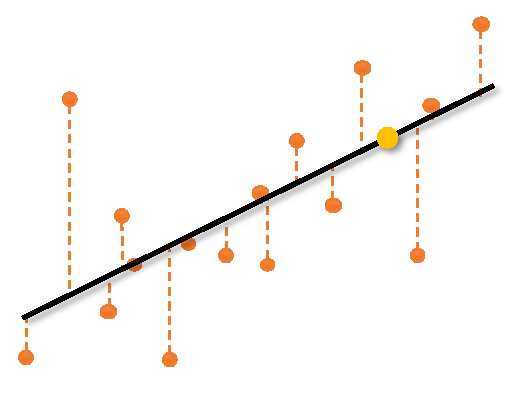
\includegraphics[width=.9\linewidth]{images/Figs/lin.pdf} } 
  \subcaption{\textbf{LIN}}
  \label{fig:lin}
\end{subfigure}
\begin{subfigure}[t]{.35\textwidth}
  \centering
  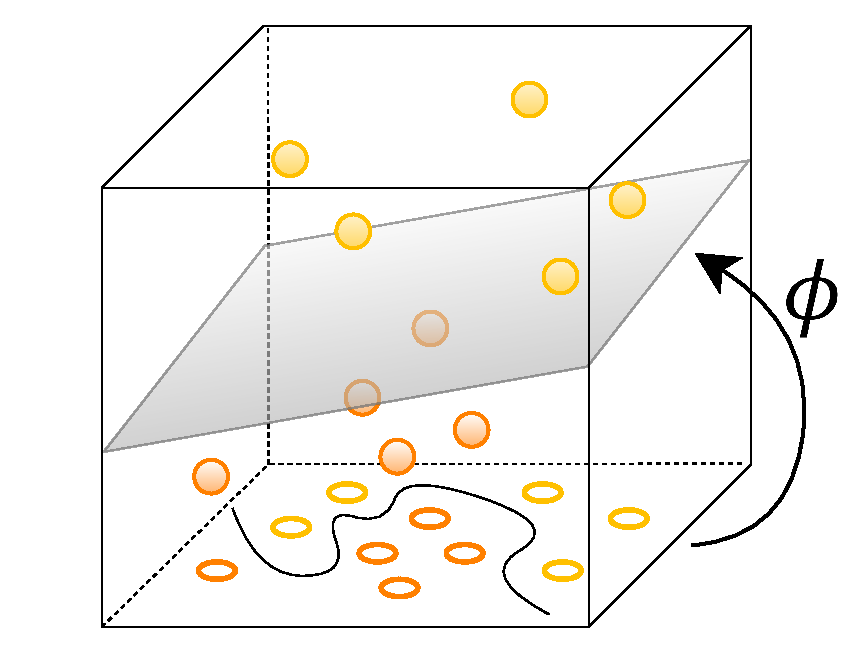
\includegraphics[width=.9\linewidth]{images/Figs/SVM.pdf} 
  \subcaption{\textbf{SVM}}
  \label{fig:svm}
\end{subfigure}
\begin{subfigure}[t]{.35\textwidth}
  \centering
  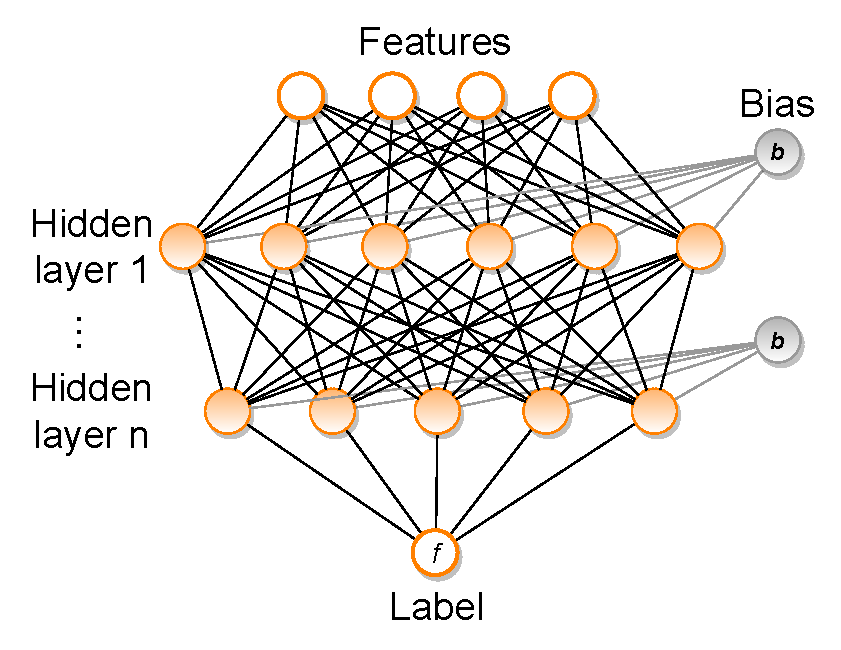
\includegraphics[width=.95\linewidth]{images/Figs/ANN.pdf}
  \subcaption{\textbf{ANN}}
  \label{fig:ann}
\end{subfigure}
} \\ \vspace{.25cm}
\makebox[\linewidth][c]{
\begin{subfigure}[t]{.3\textwidth}
  \centering
  \fbox{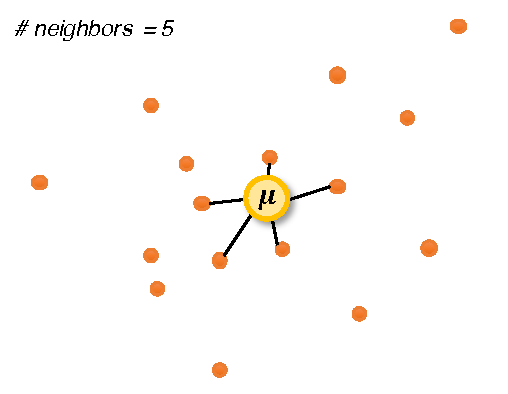
\includegraphics[width=.9\linewidth]{images/Figs/knn.pdf} }
  \subcaption{\textbf{KNN}}
  \label{fig:knn}
\end{subfigure}
\begin{subfigure}[t]{.35\textwidth}
  \centering
  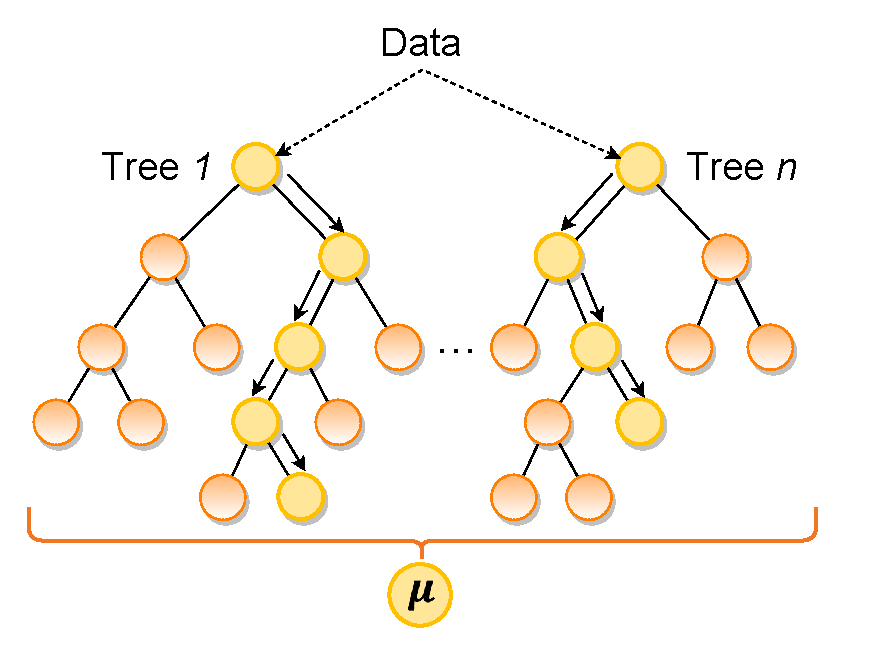
\includegraphics[width=.95\linewidth]{images/Figs/RF.pdf}
  \subcaption{\textbf{RF}}
  \label{fig:rf}
\end{subfigure}
\begin{subfigure}[t]{.35\textwidth}
  \centering
  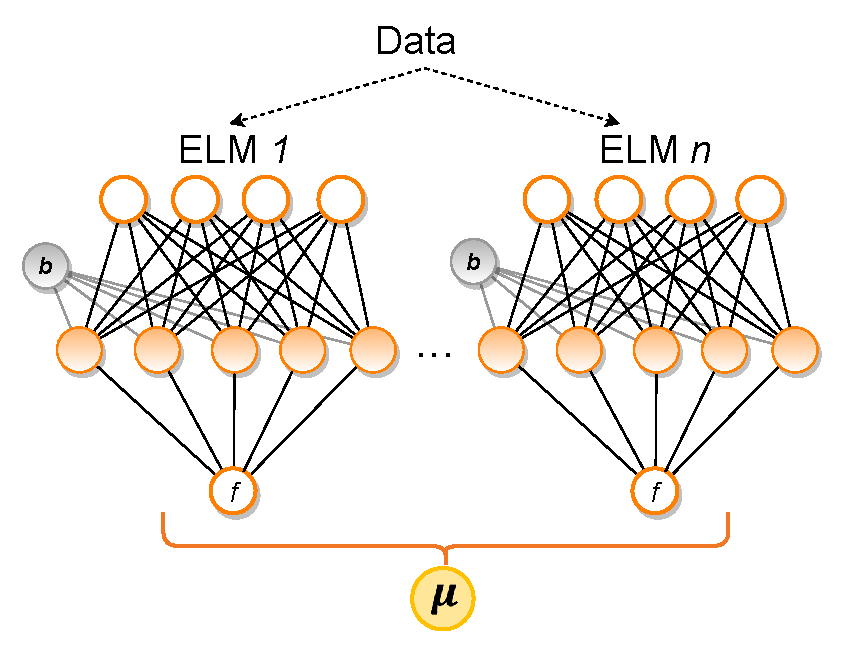
\includegraphics[width=.95\linewidth]{images/Figs/ELM_E.pdf}
  \subcaption{\textbf{ELM-E}}
  \label{fig:elme}
\end{subfigure}
}
\caption{Visualisation of ML algorithms used in this work. The selected algorithms are (a) Linear regression (LIN), (b) K-Nearest Neighbor Regression (KNN), (c) Support Vector Machine (SVM), (d) Random Forest (RF), (e) Artificial Neural Network (ANN), (f) Extreme Learning Machine Ensemble (ELM-E).}
\label{fig:ml_algorithms}
\end{figure}

\textbf{Linear Regression }(Fig. \ref{fig:lin}) assumes that the target is a linear function of the inputs. The prediction is obtained from the linear combination of the features which minimizes the residual sum of squares between the target and predicted values. It is fast and requires no tuning of hyper-parameters but shows a low accuracy for non-linear problems. The equivalent classification apporach for the linear regression is logistic regression, which estimates the probability of a data sample to belong to a specific class.

\textbf{K-nearest Neighbor Regression} (Fig. \ref{fig:knn}) is an interpolation algorithm, which computes a prediction as the average of the targets of the $k$ training samples whose features are closest to the given inputs. In classification, the average is replaced by a "majority voting" of the $k$ neighbours. The training dataset works as a look-up table for the predictions, which makes it effective for low-dimensional problems but inefficient for large datasets. We use the Euclidean distance as a measure of “closeness” and tune the number of neighbors ($k$).

\textbf{Support Vector Machine} (Fig. \ref{fig:svm}), introduced by \citet{cortes_support-vector_1995}, is the most popular algorithm in the family of kernel methods. It exploits the \textit{kernel trick}, which projects the features to a higher-dimensional space that allows for linear modelling. Its structure makes it particularly effective for high-dimensional problems, but it does not scale well with the number of samples. In this work, we use $\varepsilon$-Support Vector Regression with a radial basis function as kernel and tune the kernel coefficient ($\gamma$), the penalty parameter (C) and the error tolerance ($\varepsilon$).

\textbf{Random Forest} (Fig. \ref{fig:rf}) is an ensemble (i.e. an aggregation) of decision trees, which was proposed by \citet{breiman_random_2001}. Each of the decision trees in the ensemble pass a training sample along a set of nodes based on a threshold (defined during training) until a leaf node is reached. The prediction of each tree is obtained by averaging (or majority voting) the target values in the respective leaves. It is a popular algorithm due to its good predictive power and high robustness. Its main hyper-parameters are the number of features considered for the optimization of each threshold ($m_{ftrs}$), the minimum number of samples in each leaf ($m_{leaf}$) and the number of trees in the ensemble ($n_{est}$).
% A COMMENT ON FEATURE IMPORTANCE

\textbf{Artificial Neural Networks} (Fig. \ref{fig:ann}) consist of multiple layers of neurons, which are connected to the previous and the next layer through edges \cite{rumelhart_learning_1986}. From the input layer, which contains one neuron for each input, the data samples are passed through one or more hidden layers to the output layer with one neuron for each output. Each neuron computes a weighted linear combination of all nodes of the previous layer (for fully connected networks), which is then passed through a non-linear activation function. The weights within the network are optimised using a backpropagation procedure \cite{lecun_efficient_2012}. The hyperparameters of the ANN include the network architecture, namely the number of hidden layers and the number of neurons in each layer, the selected nonlinear activation function and a regularisation term.  

\textbf{Extreme Learning Machine Ensemble }(Fig. \ref{fig:elme}) is a collection of single-layer neural networks (ELMs), which were developed by \citet{huang_extreme_2006}. Each ELM consists of a single hidden layer, which is trained a more efficient way than traditional neural networks (see above) by a single-step optimization using a least-squares approach, which avoids the need for back-propagation. This results in a faster training time and a low number of hyper-parameters. The aggregation of $n$ ELMs in an ensemble further increases the robustness of the model and reduces the risk of overfitting \cite{huang_trends_2015}. 
It further enables the estimation of uncertainties, as described in Section~\ref{unc_ML}.

To train the ELM ensemble, we apply a bootstrap-aggregating (bagging) approach \cite{breiman_bagging_1996} where each ensemble member is trained on one bootstrapped resample of the training data. Each bootstrap replicate is obtained by resampling the $N$ training samples $N$ times uniformly and with replacement. At the output, the predictions of each ELM are averaged to give the final estimation.
The main hyper-parameters to tune in the ELM-E are the size of the hidden layer ($m_{ELM}$) and the number of ELMs in the ensemble ($n_{ELM}$). Throughout this work, we use a sigmoid activation function, which is a common choice for regression problems \cite{huang_trends_2015}.

We use the ML implementations of the \texttt{scikit-learn} library for python \cite{pedregosa_scikit-learn:_2011} for all models except the ELM-E. As no functional open-source code for the ELM-E was available when this work was carried out, we have implemented the ELM-E ourselves (regression only) using the ELM model of the \textit{HPELM} package for python \cite{akusok_high-performance_2015}, which supports computational acceleration on graphical processing units (GPUs). 
\nomenclature[A]{GPU}{Graphical Processing Units}


% A SUBSECTION ON ENSEMBLES, OR SIMPLY TWO PARAGRAPHS

\begin{comment}
% SOURCE: ICAE conference paper
Extreme Learning Machines, as proposed by Huang et al. [11], are single-layer feed-forward neural networks which are trained using a single-step optimization. The training process of ELM is up to hundreds of times faster than the training of other machine learning algorithms [11]. For our model we aggregate \textit{M} ELM to an ensemble, as shown in Fig. 1. This is known to improve the generalization performance by reducing the risk of overfitting [6,9,12], and allows to estimate the uncertainty as described in Section 2.2. At the hidden layer of each ELM, the training points $x_i$ of dimensionality d are multiplied by the randomly chosen input weights w and added to the random bias b. An activation function ƒ( ) is applied to the resulting random projections for modelling nonlinear behaviour of the data. We use a sigmoid activation function in this study, which is a common choice for regression problems [12]. The hidden layer is multiplied by the output weights $\beta$ and summed to give the model output $\hat{y}i$ (see Eq.1). During training, only $\beta$ needs to be optimized.

For ensemble training, we apply a bootstrap-aggregating (bagging) approach [13] where each ensemble member is trained on one bootstrapped resample of the training data. Each bootstrap replicate is obtained by resampling the N training samples N times uniformly and with replacement. On average, every replicate contains 63.2\% of the original data, with some duplicated samples. At the output, the predictions $\hat{y}_\mathrm{i}^\mathrm{m}$ of each ELM are averaged to give the final estimation $\hat{y}_i$ as shown in Eq. 2. The generation of M bootstrap replicates comes at a computational cost. For the implementation of each ELM, we therefore use the python toolbox \textit{hpelm} with GPU acceleration [14]. This showed significant speed-up in performance compared to the standard CPU implementation. This implementation allows us to train and to test ELM ensembles with a large number of hidden neurons on our large environmental dataset.

\begin{equation}
\label{eq:elm}
\hat{y}_{i}^{m}=\sum_{j=1}^{L} \beta_{j}^{m} f\left(\mathbf{w}_{j}^{m} \mathbf{x}_{i}+b_{j}^{m}\right), \quad \mathbf{x}_{i} \in \mathbb{R}^{d}, \mathbf{w}^{m} \in \mathbb{R}^{L \times d}, \quad i=1, \ldots, N, \quad m=1, \ldots, M
\end{equation}

\begin{equation}
\label{eq:elm_mean}
\hat{y}_{i}=\frac{1}{M} \sum_{m=1}^{M} \hat{y}_{i}^{m}, \quad i=1, \ldots, N
\end{equation}

\section{Clustering}
\textbf{K-means clustering.}

\textbf{Density-Based Spatial Clustering of Applications with Noise (DBSCAN).}
\end{comment}


\section{Uncertainties}
\subsection{Uncertainty estimation for ensemble models}
\label{unc_ML}

% SOURCE: Initial submission PV paper
The ensemble structure of both ML ensemble algorithms used in this work (RF and ELM-E) permits the estimation of uncertainties arising from the modelling process (model uncertainty, $\hat{\sigma}_M$). The remaining residuals after the subtraction of the model variance are further used to estimate the uncertainty related to the data noise (data uncertainty, $\hat{\sigma}_D$) \cite{akusok_per-sample_2019,guignard_uncertainty_2020}. 
% This approach enables a specific characterization of the uncertainty for each spatio-temporal point.
It has been previously used to estimate for example wind speeds for wind power generation~\cite{wan_probabilistic_2014}.

The ensemble method is based on a bagging (bootstrap-aggregating) approach, which introduces randomness into the model  \cite{breiman_bagging_1996}.
Every ensemble member is trained on one bootstrapped resample of the training data, which is
obtained by sampling the training set uniformly and with replacement.
On average, every such resample contains 63.2\% of the original data, with some duplicated samples \cite{breiman_bagging_1996}. 
The model uncertainty is quantified as the standard deviation of the predictions of all model in the ensemble, which is computed as \cite{heskes_practical_1997}:

\begin{equation}
\label{eq:model_unc}
  \hat{\sigma}_M^2 (\mathbf{x}_i) = \frac{1}{N} \sum_{n=1}^N (\hat{y}_i^n - \hat{y}_i)^2, \quad i=1,...,L
\end{equation}

where $\hat{\sigma}_M$ denotes the model standard deviation, referred to as model uncertainty, $N$ denotes the ensemble length, $\hat{y}_i$ is the ensemble prediction for sample $\mathbf{x}_i$ and $\hat{y}_i^n$ is the prediction of ensemble member $n$.

Additionally to the model variance, we estimate the variance of the data noise by modelling the remaining residuals. They are derived by subtracting the model variance from the squared difference between $\hat{y}_i$ and the targets $t_i$, as shown below.
In order to reduce bias, the out-of-bag (OOB) model output are used, which is the mean of the ensemble members for which a given training data point was not considered (due to bootstrapping) \cite{heskes_practical_1997}. 

\begin{equation}
\label{eq:data_unc}
  \hat{\sigma}_D^2 (\mathbf{x}_i) = \max \left\{ (t_i - \hat{y}_i)^2 - \hat{\sigma}_M^2 (\mathbf{x}_i) , 0 \right\}, \quad i=1,...,L
\end{equation}
 
 where $\hat{\sigma}_D$ denotes the standard deviation of data noise, referred to as data uncertainty, and $t_i$ is the target value for sample $\mathbf{x}_i$. 
$\hat{\sigma}_D$ can only be computed if $t_i$ is known. Thus, a second ML model is trained from the residuals to predict $\hat{\sigma}_D$ for points with unknown targets. Unless mentioned otherwise, the same hyper-parameters are used in both models.

The total variance of a variable that is estimated using a ML model is the squared sum of its model uncertainty and its data uncertainty: 

\begin{equation}
\label{eq:total_unc}
\sigma^2 (\mathbf{x}_i) = \hat{\sigma}_M^2 (\mathbf{x}_i) + \hat{\sigma}_D^2 (\mathbf{x}_i), \quad i=1,...,L
\end{equation}

% Source: ICAE paper
% Applying bagging to the ELM ensemble increases the quality of the prediction and it also allows to compute the model uncertainty $\hat{\sigma}M$, derived from the variance ${\hat{\sigma}}_M^2$ of the M model outputs ${\hat{y}}_\mathrm{i}^\mathrm{m}$ (see Eq. 3) [9,15]. Afterwards, remaining residuals are derived by subtracting the model variance from the squared difference between the model outputs and the targets ti, as visible in Eq. 4. We compute these residuals for the training data, which are used to train a second ELM ensemble. The output is the data noise variance ${\hat{\sigma}}_D^2$, and the standard deviation $\hat{\sigma}D$ quantifies the data uncertainty. Adding model and data noise variance provides a qualitative estimate of the uncertainty on the predictions.

\begin{comment}
\subsubsection{Uncertainty for GIS methods}

The uncertainty for the GIS-derived and bias corrected quantities, namely $S_{sh}$ and $SVF$, is estimated from the residuals between the values computed using the $(2 \times 2)m^2$ and the $(0.5 \times 0.5)m^2$ resolution DSM in Geneva. The latter is considered the "true" surface model. 
The error in the GIS-derived quantities is treated as a random variable, whose first and second moments are estimated from the mean and the variance of the discrepancy. The mean is used for the bias correction, as explained in Sections \ref{shade} and \ref{svf}, while the variance represents the uncertainty.

It should be noted that the error of the GIS methods for $C_{sh}$ and $C_{pv}$ are not computed in the way described here, as they form part of the data uncertainty estimated by the subsequent ML models.
\end{comment}

\subsection{Uncertainty propagation}
\label{method_unc_prop}

For the estimation of renewable resource potential, different sources of uncertainties must be combined and propagated through physicals models. 
For this propagation of uncertainties, the correlation among the random variables plays a key role.
%
% SOURCE: Initial submission PV paper
% The correlation among the random variables plays a key role in the propagation of uncertainty. 
If statistical independence can be assumed, the mean and variance of the resulting variables can be computed from the mean and variance of each parameter only, which greatly simplifies the uncertainty propagation.
However, this assumption does not always hold, in which case correlations between random variables must be taken into account.
% As the uncertainty is computed separately for each spatio-temporal data point, we assume statistical independence between meteorological and building related parameters, namely between $G_h, G_B, G_D$ and $S_{sh}, SVF, A_{PV}$. This is valid as the uncertainty of the horizontal radiation is dominated by the meteorological conditions, while those of $S_{sh}(t), SVF, A_{PV}$ are related to the GIS and ML methods. These are independent and uncorrelated processes.
In the context of this thesis, we consider the propagation of uncertainties over a set of sums and products of random variables using error propagation theory \cite{jcgm_evaluation_2008, goodman_variance_1962}. This section summarises the error propagation formulas for summations and multiplications, applied in the following chapters, in their general form.

% In error propagation theory~\cite{jcgm_evaluation_2008, goodman_variance_1962}, the uncertainty on any final measurand is the result of the propagation over a set of sums and products of its variables. 
In error analysis, the variance of the sum of $N$ randomly distributed variables $X_i$ is given by:

\begin{equation}
\label{eq:unc_sum}
\mathrm{Var}\left(\sum_{i=1}^N X_i\right) = \sum_{i=1}^N\mathrm{Var}(X_i) + 2\sum_{i < j}\mathrm{Cov}(X_i, X_j)
\end{equation}
which simplifies to the sum of the variances of $X_i$ if the random variables are statistically independent.
%
The variance of the product of two random variables $X$ and $Y$ is defined as:

\begin{align}
\label{eq:var_mult_corr}
\mathrm{Var}(X Y)&=E\left(X^{2} Y^{2}\right)-E(X Y)^{2} \\
&= \mathrm{Cov}\left(X^{2}, Y^{2}\right)+\left[\mathrm{Var}(X)+\mathrm{E}(X)^{2}\right] \left[\mathrm{Var}(Y)+\mathrm{E}(Y)^{2}\right]-[\mathrm{Cov}\left(X, Y\right)+\mathrm{E}(X)  \mathrm{E}(Y)]^{2} \nonumber
\end{align}

If statistical independence between the random variables $X$ and $Y$can be assumed, the terms $\mathrm{Cov}\left(X^{2}, Y^{2}\right)$and $\mathrm{Cov}\left(X, Y\right)$ can be omitted, such that Eq.~\ref{eq:var_mult_corr} becomes a function of the variances of $X$ and $Y$ and their expected value:
\begin{equation}
\label{eq:unc_prod}
\mathrm{Var}(XY) = \mathrm{Var}(X)\mathrm{Var}(Y) + \mathrm{Var}(X) \mathrm{E}(Y)^2 + \mathrm{Var}(Y) \mathrm{E}(X)^2
\end{equation}
%% ADD FULL EQUATION WITH COVARIANCES